\subsection{Question 1}

\begin{figure}[H]
  \centering
  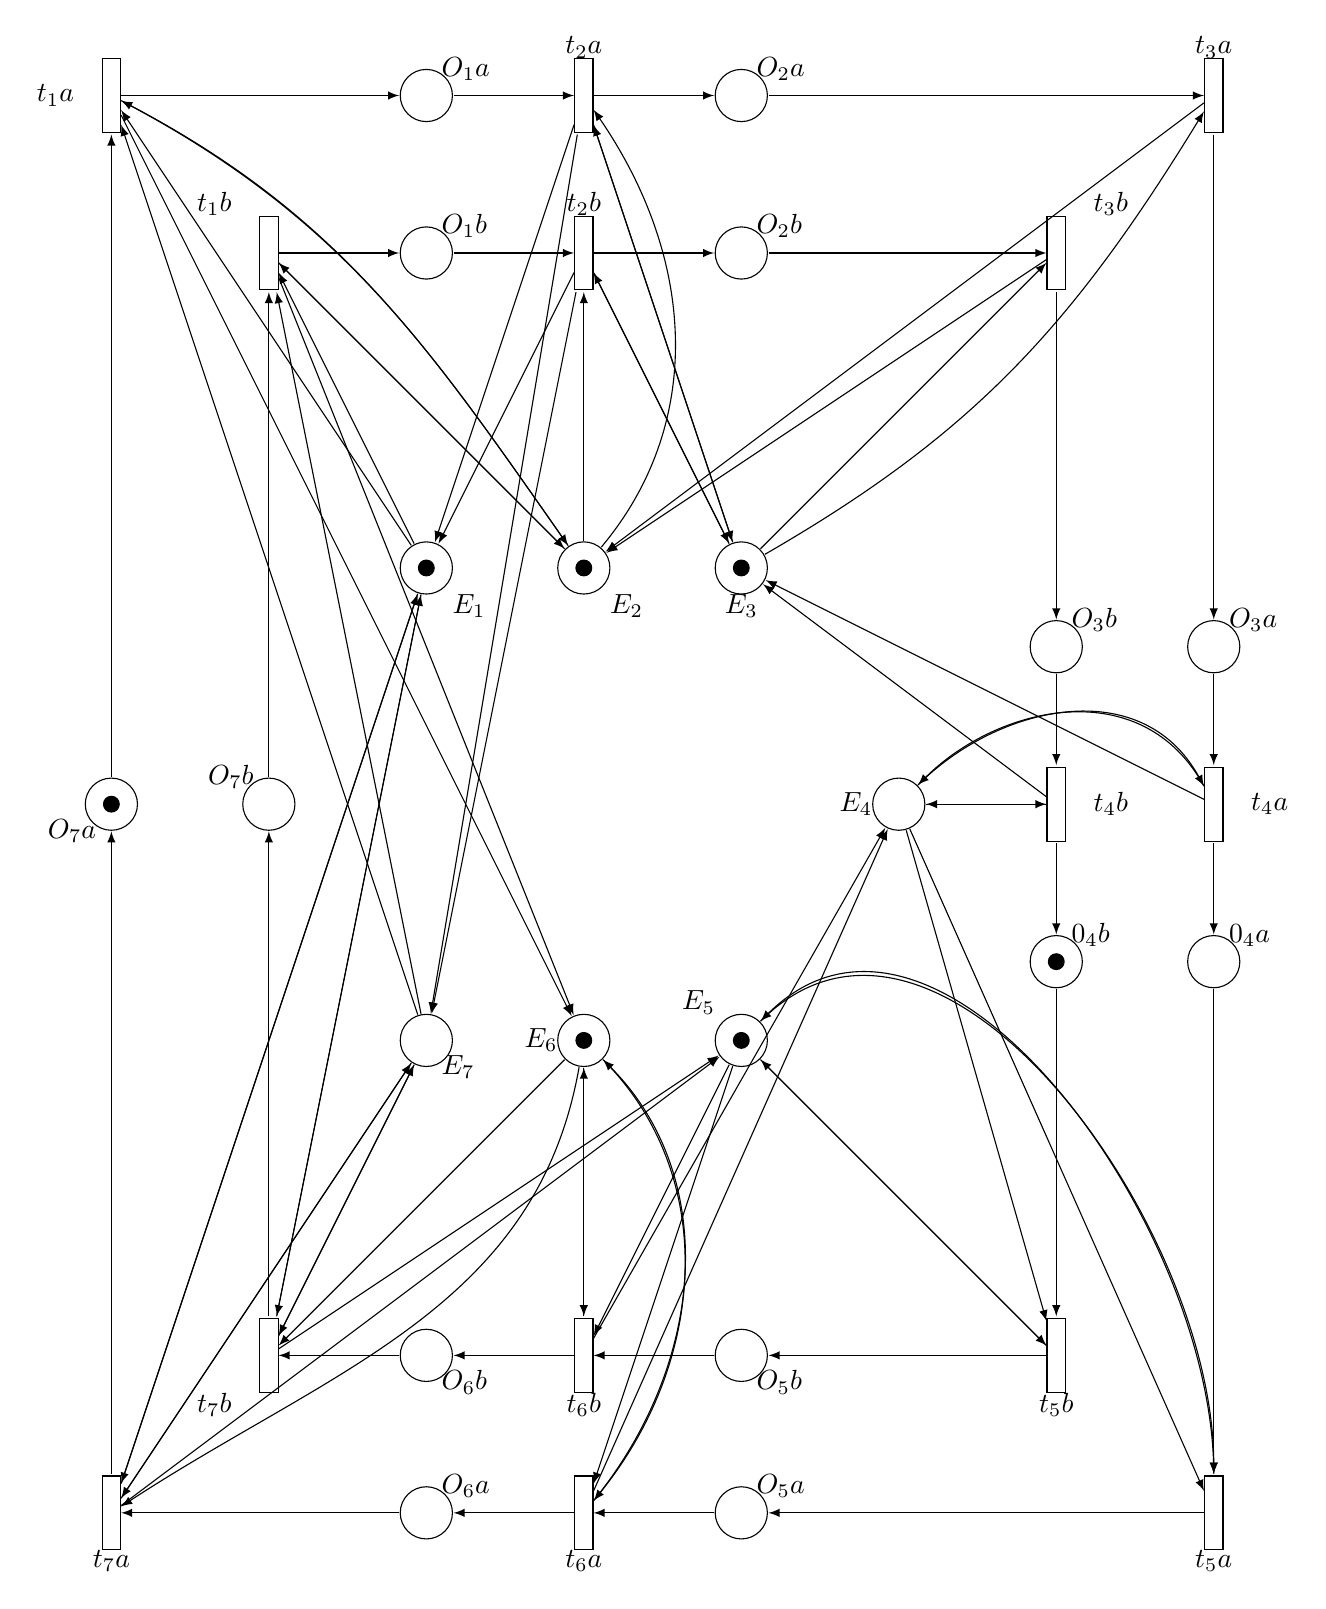
\begin{tikzpicture}
    % Liste des places
    \draw (-9,0) node[below left = 2pt] {$O_7a$};
    \node[draw,circle,scale=2] (o7a) at (-9, 0) {};

    \draw (-7,0) node[above left = 2pt] {$O_7b$};
    \node[draw,circle,scale=2] (o7b) at (-7, 0) {};

    \draw (-5, -7) node[below right = 2pt] {$O_6b$};
    \node[draw,circle,scale=2] (o6b) at (-5, -7) {};

    \draw (-5,-9) node[above right = 2pt] {$O_6a$};
    \node[draw,circle,scale=2] (o6a) at (-5, -9) {};

    \draw (-5,-3) node[below right = 2pt] {$E_7$};
    \node[draw,circle,scale=2] (e7) at (-5, -3) {};

    \draw (-5,3) node[below right = 6pt] {$E_1$};
    \node[draw,circle,scale=2] (e1) at (-5, 3) {};

    \draw (-5,7) node[above right = 2pt] {$O_1b$};
    \node[draw,circle,scale=2] (o1b) at (-5, 7) {};

    \draw (-5,9) node[above right = 2pt] {$O_1a$};
    \node[draw,circle,scale=2] (o1a) at (-5, 9) {};

    \draw (-3,3) node[below right = 6pt] {$E_2$};
    \node[draw,circle,scale=2] (e2) at (-3, 3) {};

    \draw (-3,-3) node[left = 6pt] {$E_6$};
    \node[draw,circle,scale=2] (e6) at (-3, -3) {};

    \draw (-1, -7) node[below right = 2pt] {$O_5b$};
    \node[draw,circle,scale=2] (o5b) at (-1, -7) {};

    \draw (-1,-9) node[above right = 2pt] {$O_5a$};
    \node[draw,circle,scale=2] (o5a) at (-1, -9) {};

    \draw (-1,-3) node[above left = 6pt] {$E_5$};
    \node[draw,circle,scale=2] (e5) at (-1, -3) {};

    \draw (-1,3) node[below = 6pt] {$E_3$};
    \node[draw,circle,scale=2] (e3) at (-1, 3) {};

    \draw (-1,7) node[above right = 2pt] {$O_2b$};
    \node[draw,circle,scale=2] (o2b) at (-1, 7) {};

    \draw (-1,9) node[above right = 2pt] {$O_2a$};
    \node[draw,circle,scale=2] (o2a) at (-1, 9) {};

    \draw (1,0) node[left = 6pt] {$E_4$};
    \node[draw,circle,scale=2] (e4) at (1, 0) {};

    \draw (3,2) node[above right = 2pt] {$O_3b$};
    \node[draw,circle,scale=2] (o3b) at (3, 2) {};

    \draw (3,-2) node[above right = 2pt] {$0_4b$};
    \node[draw,circle,scale=2] (o4b) at (3, -2) {};

    \draw (5,2) node[above right = 2pt] {$O_3a$};
    \node[draw,circle,scale=2] (o3a) at (5, 2) {};

    \draw (5,-2) node[above right = 2pt] {$0_4a$};
    \node[draw,circle,scale=2] (o4a) at (5, -2) {};







    % Liste des transitions
    \draw (-9,9) node[left = 10pt] {$t_1a$};
    \node[draw,rectangle,yscale=4] (t1a) at (-9, 9) {};

    \draw (-7,7) node[above left = 10pt] {$t_1b$};
    \node[draw,rectangle,yscale=4] (t1b) at (-7, 7) {};

    \draw (-3,9) node[above = 10pt] {$t_2a$};
    \node[draw,rectangle,yscale=4] (t2a) at (-3, 9) {};

    \draw (-3,7) node[above = 10pt] {$t_2b$};
    \node[draw,rectangle,yscale=4] (t2b) at (-3, 7) {};

    \draw (5,9) node[above = 10pt] {$t_3a$};
    \node[draw,rectangle,yscale=4] (t3a) at (5, 9) {};

    \draw (3,7) node[above right = 10pt] {$t_3b$};
    \node[draw,rectangle,yscale=4] (t3b) at (3, 7) {};

    \draw (3,0) node[right = 10pt] {$t_4b$};
    \node[draw,rectangle,yscale=4] (t4b) at (3, 0) {};

    \draw (5,0) node[right = 10pt] {$t_4a$};
    \node[draw,rectangle,yscale=4] (t4a) at (5, 0) {};

    \draw (5,-9) node[below = 10pt] {$t_5a$};
    \node[draw,rectangle,yscale=4] (t5a) at (5, -9) {};

    \draw (3,-7) node[below = 10pt] {$t_5b$};
    \node[draw,rectangle,yscale=4] (t5b) at (3, -7) {};

    \draw (-3,-9) node[below = 10pt] {$t_6a$};
    \node[draw,rectangle,yscale=4] (t6a) at (-3, -9) {};

    \draw (-3, -7) node[below = 10pt] {$t_6b$};
    \node[draw,rectangle,yscale=4] (t6b) at (-3, -7) {};

    \draw (-9,-9) node[below = 10pt] {$t_7a$};
    \node[draw,rectangle,yscale=4] (t7a) at (-9, -9) {};

    \draw (-7,-7) node[below left = 10pt] {$t_7b$};
    \node[draw,rectangle,yscale=4] (t7b) at (-7, -7) {};



    % Liste des arcs
    \draw[->,>=latex] (t1a) -- (o1a);

    \draw[->,>=latex] (o1a) -- (t2a);

    \draw[->,>=latex] (t2a) -- (o2a);

    \draw[->,>=latex] (o2a) -- (t3a);

    \draw[->,>=latex] (t3a) -- (o3a);

    \draw[->,>=latex] (o3a) -- (t4a);

    \draw[->,>=latex] (t4a) -- (o4a);

    \draw[->,>=latex] (o4a) -- (t5a);

    \draw[->,>=latex] (t5a) -- (o5a);

    \draw[->,>=latex] (o5a) -- (t6a);

    \draw[->,>=latex] (t6a) -- (o6a);

    \draw[->,>=latex] (o6a) -- (t7a);

    \draw[->,>=latex] (t7a) -- (o7a);

    \draw[->,>=latex] (o7a) -- (t1a);



    \draw[->,>=latex] (t1b) -- (o1b);

    \draw[->,>=latex] (o1b) -- (t2b);

    \draw[->,>=latex] (t2b) -- (o2b);

    \draw[->,>=latex] (o2b) -- (t3b);

    \draw[->,>=latex] (t3b) -- (o3b);

    \draw[->,>=latex] (o3b) -- (t4b);

    \draw[->,>=latex] (t4b) -- (o4b);

    \draw[->,>=latex] (o4b) -- (t5b);

    \draw[->,>=latex] (t5b) -- (o5b);

    \draw[->,>=latex] (o5b) -- (t6b);

    \draw[->,>=latex] (t6b) -- (o6b);

    \draw[->,>=latex] (o6b) -- (t7b);

    \draw[->,>=latex] (t7b) -- (o7b);

    \draw[->,>=latex] (o7b) -- (t1b);



    \draw[->,>=latex] (e1) -- (t1b);

    \draw[->,>=latex] (e1) -- (t1a);

    \draw[->,>=latex] (e1) -- (t7a);

    \draw[->,>=latex] (e1) -- (t7b);

    \draw[->,>=latex] (t7a) -- (e1);

    \draw[->,>=latex] (t7b) -- (e1);

    \draw[->,>=latex] (t2a) -- (e1);

    \draw[->,>=latex] (t2b) -- (e1);


    \draw[->,>=latex] (e2) -- (t2b);

    \draw[->,>=latex] (e2) to[out=50,in=-50] (t2a);

    \draw[->,>=latex] (e2) to[out=125,in=-25] (t1a);

    \draw[->,>=latex] (e2) -- (t1b);

    \draw[->,>=latex] (t1a) to[out=-25,in=125] (e2);

    \draw[->,>=latex] (t1b) -- (e2);

    \draw[->,>=latex] (t3a) -- (e2);

    \draw[->,>=latex] (t3b) -- (e2);


    \draw[->,>=latex] (e3) -- (t3b);

    \draw[->,>=latex] (e3) to[out=30,in=-125] (t3a);

    \draw[->,>=latex] (e3) -- (t2a);

    \draw[->,>=latex] (e3) -- (t2b);

    \draw[->,>=latex] (t2a) -- (e3);

    \draw[->,>=latex] (t2b) -- (e3);

    \draw[->,>=latex] (t4a) -- (e3);

    \draw[->,>=latex] (t4b) -- (e3);


    \draw[->,>=latex] (e4) -- (t5b);

    \draw[->,>=latex] (e4) -- (t5a);

    \draw[->,>=latex] (e4) to[out=45,in=125] (t4a);

    \draw[->,>=latex] (e4) -- (t4b);

    \draw[->,>=latex] (t4a) to[out=125,in=45] (e4);

    \draw[->,>=latex] (t4b) -- (e4);

    \draw[->,>=latex] (t6a) -- (e4);

    \draw[->,>=latex] (t6b) -- (e4);


    \draw[->,>=latex] (e5) -- (t6b);

    \draw[->,>=latex] (e5) -- (t6a);

    \draw[->,>=latex] (e5) to[out=45,in=90] (t5a);

    \draw[->,>=latex] (e5) -- (t5b);

    \draw[->,>=latex] (t5a) to[out=90,in=45] (e5);

    \draw[->,>=latex] (t5b) -- (e5);

    \draw[->,>=latex] (t7a) -- (e5);

    \draw[->,>=latex] (t7b) -- (e5);


    \draw[->,>=latex] (e6) -- (t7b);

    \draw[->,>=latex] (e6) to[out=-100,in=30] (t7a);

    \draw[->,>=latex] (e6) to[out=-45,in=45] (t6a);

    \draw[->,>=latex] (e6) -- (t6b);

    \draw[->,>=latex] (t6a) to[out=45,in=-45] (e6);

    \draw[->,>=latex] (t6b) -- (e6);

    \draw[->,>=latex] (t1a) -- (e6);

    \draw[->,>=latex] (t1b) -- (e6);


    \draw[->,>=latex] (e7) -- (t1b);

    \draw[->,>=latex] (e7) -- (t1a);

    \draw[->,>=latex] (e7) -- (t7a);

    \draw[->,>=latex] (e7) -- (t7b);

    \draw[->,>=latex] (t7a) -- (e7);

    \draw[->,>=latex] (t7b) -- (e7);

    \draw[->,>=latex] (t2a) -- (e7);

    \draw[->,>=latex] (t2b) -- (e7);






    %\draw[->,>=latex] (po) to[out=135,in=-135] (t1);

    % Marquage
    \draw [fill](-5,3) circle (0.1) ;
    \draw [fill](-3,3) circle (0.1) ;
    \draw [fill](-3,-3) circle (0.1) ;
    \draw [fill](-1,-3) circle (0.1) ;
    \draw [fill](-1,3) circle (0.1) ;
    \draw [fill](3,-2) circle (0.1) ;
    \draw [fill](-9,0) circle (0.1) ;




  \end{tikzpicture}
    \caption{Rp de la question 12.1} \label{fig:M1}
\end{figure}

Un train ce trouvant dans la le secteur i voulant avancer, il faut que le secteur i+1 et i+2 soient libres.
Cela equivaux a actioner la transition ti+1, qui verifie que les places Ei+1 et Ei+2 contienent des jetons.
Ensuite, le secteur i est libéré, le secteur i+1 occupé et le secteur i+2 inchangé.
Cela equivaux a mettre un jeton dans la place Ei, enlever un jeton de la place Ei+1 et le rajouter dans $O_{a_i+1}$.
Pour continuer, le train doit verrifier que les secteurs i+2 et i+3 sont libres il libère alors i+1, i+2 devient occupé et i+3 reste inchangé.
Ce motif se repete autant de fois que le train veux changer de secteur.

\subsection{Question 2}
\begin{figure}[H]
  \centering
  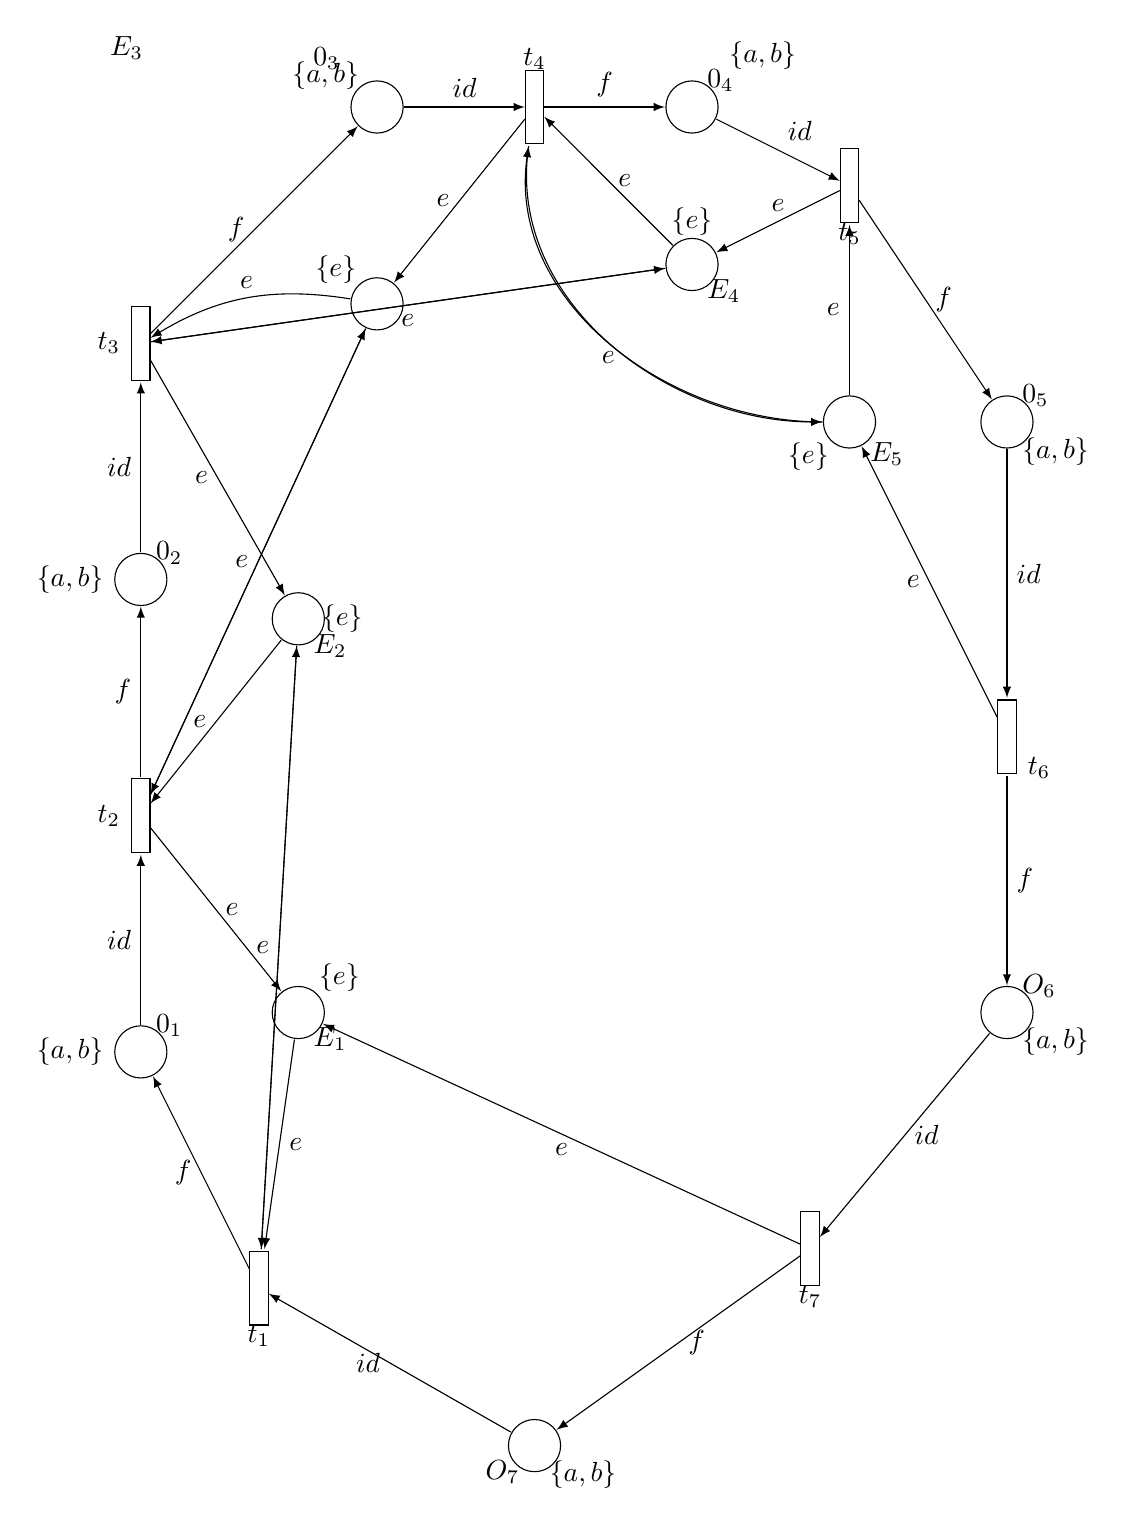
\begin{tikzpicture}

    % Liste des places
    \draw (0,-8) node[below left = 2pt] {$O_7$};
    \draw (0,-8) node[below right = 2pt] {$\{a,b\}$};
    \node[draw,circle,scale=2] (o7) at (0, -8) {};
    \draw (6,-2.5) node[above right = 2pt] {$O_6$};
    \draw (6,-2.5) node[below right = 2pt] {$\{a,b\}$};
    \node[draw,circle,scale=2] (o6) at (6, -2.5) {};
    \draw (6,5) node[above right = 2pt] {$0_5$};
    \draw (6,5) node[below right = 2pt] {$\{a,b\}$};
    \node[draw,circle,scale=2] (o5) at (6, 5) {};
    \draw (2,9) node[above right = 2pt] {$0_4$};
    \draw (2,9) node[above right = 10pt] {$\{a,b\}$};
    \node[draw,circle,scale=2] (o4) at (2, 9) {};
    \draw (-2,9) node[above left = 10pt] {$0_3$};
    \draw (-2,9) node[above left = 3pt] {$\{a,b\}$};
    \node[draw,circle,scale=2] (o3) at (-2, 9) {};
    \draw (-5,3) node[above right = 2pt] {$0_2$};
    \draw (-5,3) node[left = 10pt] {$\{a,b\}$};
    \node[draw,circle,scale=2] (o2) at (-5, 3) {};
    \draw (-5,-3) node[above right = 2pt] {$0_1$};
     \draw (-5,-3) node[left = 10pt] {$\{a,b\}$};
    \node[draw,circle,scale=2] (o1) at (-5, -3) {};
    \draw (-3,-2.5) node[below right = 2pt] {$E_1$};
    \draw (-3,-2.5) node[above right = 4pt] {$\{e\}$};
    \node[draw,circle,scale=2] (e1) at (-3, -2.5) {};
	\draw (-3,2.5) node[below right = 2pt] {$E_2$};
	\draw (-3,2.5) node[right = 5pt] {$\{e\}$};
    \node[draw,circle,scale=2] (e2) at (-3, 2.5) {};
    \draw (-2,6.5) node[below right = -100pt] {$E_3$};
    \draw (-2,6.5) node[above left = 4pt] {$\{e\}$};
    \node[draw,circle,scale=2] (e3) at (-2, 6.5) {};
    \draw (2, 7) node[below right = 2pt] {$E_4$};
    \draw (2,7) node[above = 7pt] {$\{e\}$};
    \node[draw,circle,scale=2] (e4) at (2, 7) {};
    \draw (4,5) node[below right = 4pt] {$E_5$};
    \draw (4,5) node[below left = 4pt] {$\{e\}$};
    \node[draw,circle,scale=2] (e5) at (4, 5) {};

    % Liste des transitions
    \draw (-3.5,-6) node[below = 10pt] {$t_1$};
    \node[draw,rectangle,yscale=4] (t1) at (-3.5, -6) {};
    \draw (-5,0) node[left = 4pt] {$t_2$};
    \node[draw,rectangle,yscale=4] (t2) at (-5, 0) {};
    \draw (-5,6) node[left = 4pt] {$t_3$};
    \node[draw,rectangle,yscale=4] (t3) at (-5, 6) {};
    \draw (0,9) node[above = 10pt] {$t_4$};
    \node[draw,rectangle,yscale=4] (t4) at (0, 9) {};
    \draw (4,8) node[below = 10pt] {$t_5$};
    \node[draw,rectangle,yscale=4] (t5) at (4, 8) {};
    \draw (6,1) node[below right = 4pt] {$t_6$};
    \node[draw,rectangle,yscale=4] (t6) at (6, 1) {};
    \draw (3.5,-5.5) node[below = 10pt] {$t_7$};
    \node[draw,rectangle,yscale=4] (t7) at (3.5, -5.5) {};

    % Liste des arcs
    \draw[->,>=latex] (o7) -- (t1) node[midway, left]{$id$};
    \draw[->,>=latex] (t1) -- (o1) node[midway, left]{$f$};
    \draw[->,>=latex] (o1) -- (t2) node[midway, left]{$id$};
    \draw[->,>=latex] (t2) -- (o2) node[midway, left]{$f$};
    \draw[->,>=latex] (o2) -- (t3) node[midway, left]{$id$};
    \draw[->,>=latex] (t3) -- (o3) node[midway, left]{$f$};
    \draw[->,>=latex] (o3) -- (t4) node[midway, above]{$id$};
    \draw[->,>=latex] (t4) -- (o4) node[midway, above]{$f$};
    \draw[->,>=latex] (o4) -- (t5) node[midway, above right]{$id$};
    \draw[->,>=latex] (t5) -- (o5) node[midway, right]{$f$};
    \draw[->,>=latex] (o5) -- (t6) node[midway, right]{$id$};
    \draw[->,>=latex] (t6) -- (o6) node[midway, right]{$f$};
    \draw[->,>=latex] (o6) -- (t7) node[midway, right]{$id$};
    \draw[->,>=latex] (t7) -- (o7) node[midway, right]{$f$};

    \draw[->,>=latex] (e1) -- (t1) node[midway, right]{$e$};
    \draw[->,>=latex] (t2) -- (e1) node[midway, right]{$e$};
    \draw[->,>=latex] (e2) -- (t1) node[midway, left]{$e$};
    \draw[->,>=latex] (t1) -- (e2);
    \draw[->,>=latex] (e3) -- (t2);
    \draw[->,>=latex] (t2) -- (e3) node[midway, left]{$e$};
    \draw[->,>=latex] (t3) -- (e2) node[midway, left]{$e$};
    \draw[->,>=latex] (e2) -- (t2) node[midway, left]{$e$};
    \draw[->,>=latex] (e3) to [bend right=20] node[midway, above]{$e$}(t3) ;
    \draw[->,>=latex] (t4) -- (e3) node[midway, left]{$e$};
    \draw[->,>=latex] (t3) -- (e4) node[midway, below]{$e$};
    \draw[->,>=latex] (e4) -- (t3);
    \draw[->,>=latex] (e4) -- (t4) node[midway, right]{$e$};
    \draw[->,>=latex] (t5) -- (e4) node[midway, above]{$e$};
    \draw[->,>=latex] (e5) to [out=-180, in=-100] node[midway, below]{$e$}(t4);
    \draw[->,>=latex] (t4) to [out=-100, in=-180] (e5);
    \draw[->,>=latex] (e5) -- (t5) node[midway, left]{$e$};
    \draw[->,>=latex] (t6) -- (e5) node[midway, left]{$e$};
    \draw[->,>=latex] (t7) -- (e1) node[midway, below]{$e$};



  \end{tikzpicture}
  \caption{Réseau de petri associé à 12.2} \label{fig:M1}
\end{figure}

\begin{center}
\begin{tabular}{|l|c|r|}
  \hline
  Function & $a + e$ & $b + e$ \\
  \hline
  $f$ & $a$ & $b$ \\
  \hline
\end{tabular}
\end{center}
